
\documentclass[a4paper, 11pt, conference]{ieeeconf}
\overrideIEEEmargins

\usepackage{graphics} % for pdf, bitmapped graphics files
\usepackage{graphicx}
%\usepackage{epsfig} % for postscript graphics files
%\usepackage{mathptmx} % assumes new font selection scheme installed
%\usepackage{times} % assumes new font selection scheme installed
%\usepackage{amsmath} % assumes amsmath package installed
%\usepackage{amssymb}  % assumes amsmath package installed
\title{\LARGE \bf Tool For Creating Online Education Courses Designed for Novice Authors }
\author{Mostafa S. Tareque, Abelardo Pardo}

%%%%%%%%%%%%%%%%%%%%%%%%%%%%%%%%%%%%%%%%%%%%%%%%%%%%%%%%%%%%%%%%%%%%%%%%%%%%%%%%

\begin{document}
\maketitle
\pagestyle{empty}
\thispagestyle{empty}

%%%%%%%%%%%%%%%%%%%%%%%%%%%%%%%%%%%%%%%%%%%%%%%%%%%%%%%%%%%%%%%%%%%%%%%%%%%%%%%%
\begin{abstract}
This paper outlines the design of a system that uses open source tools to allow any independent author to intuitively publish their educational content onto an online platform. The author can easily employ their own full-scale educational web application without having any preliminary software development experience. The platform provides student feedback via interactive visual interfaces and in turn serves as a positive reinforcement to the individual's performance. The system that feeds the visual analytics back to the individual user and the general audience is fully automated, and thus requires no assistance from the author.
\end{abstract}
%%%%%%%%%%%%%%%%%%%%%%%%%%%%%%%%%%%%%%%%%%%%%%%%%%%%%%%%%%%%%%%%%%%%%%%%%%%%%%%%

\section{INTRODUCTION}
Web based education systems are in high demand due to the end users' convenience. Existing platforms already allow students taking courses to easily access documents and resources. However the procedure for an academic author to publish their content online is not as simple as the student's experience. Existing web based platforms are run by institutions that have certain structures and constraints that must be adhered to by any contributing author. These current platforms require web developers to create the front end of the site as well as continuous management of the back end. This leads to restrictions in flexibility when designing courses as well as potential financial limitations due to the initial and ongoing management costs.

The education tool discussed in this paper will provide solutions to the issues faced by current educational web based platforms. The tool is intuitive, allowing the novice author to easily upload course material without the need to manually create or manage the site. The tool is capable of handling a large user base, and automatically generates visual analytics for each user based on their activity. 

The following sections will discuss the design of our education tool. Section II discusses the minimal contribution needed from the author in publishing the web platform, and the enhanced content that is returned by the tool. Section III outlines the automated structure of the web platform and describes in detail the flow of analytics back to the user. Lastly Section IV discusses the kinds of automatically generated visual analytics that provide constructive feedback to the user.

\section{Contribution of the Author}
The key aspect of the education tool is that it reduces the academic's contribution to a bare minimum. 
The author has to input the content onto a series of files in accordance to set guidelines that are simple enough to be intuitive. These guidelines defined in the reStructuredText format, can be learned effortlessly using online resources. As shown in Figure \ref{fig:rst} each portion of content can be classified into types of sections using markups. Educational content can be broken down into three simple sections - notes, questions and videos. Other directives, such as link to other pages, can also be inserted.

\begin{figure}
\centering
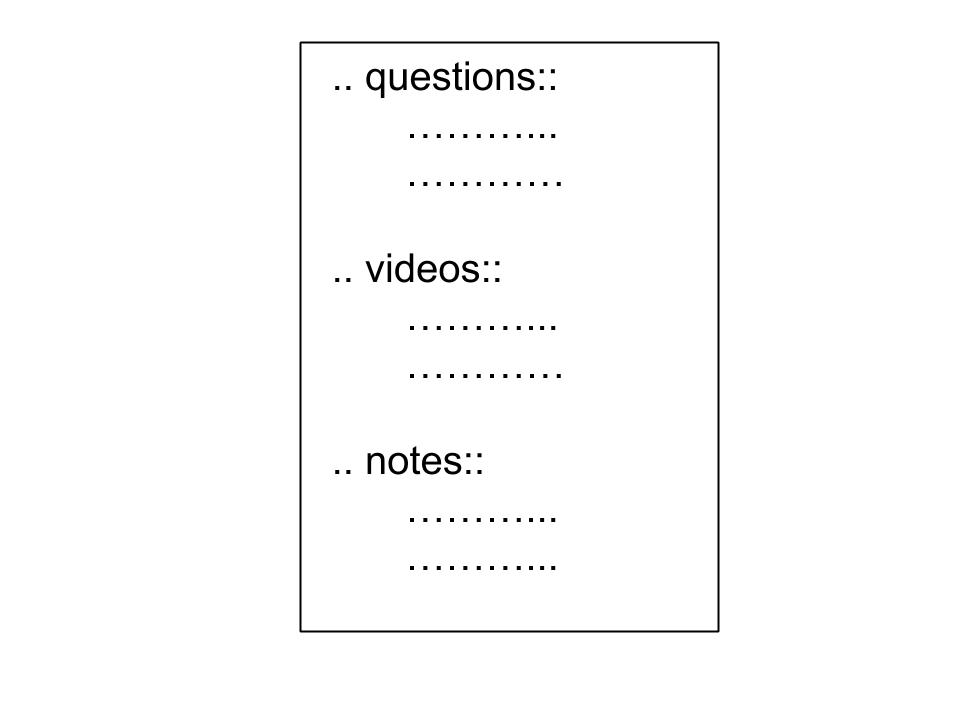
\includegraphics[width=0.4\textwidth]{rst.png}
\caption{\label{fig:rst}reStructuredText markup format}
\end{figure}

The program that executes this is Sphinx, a documentation tool for creating websites. Sphinx allows handling of custom directives using developer created extensions. Customized directives allow a simple directive tag on a reStructuredText to be converted into web content (HTML, CSS) on the page. These directives further embed JavaScript listeners on to the page to collect user meta-data and relay it to the database. The customized directives also create code that processes the corresponding meta-data to obtain visual analytics for every student that accesses it. This all happens seamlessly without the need for the author to analyze the data themselves and is referred as the back-annotation loop. To customize web design, the author is given the option to choose from one of the many templates by configuring the setting.py file. The website generated by the Sphinx tool is hosted on the worldwide web using the Django Framework.

\section{The Automated Back-Annotation Loop}

The back-annotation loop is the process by which meta-data is sent back to the user through an automated flow. As shown in Figure \ref{fig:loop} the flow initiates with the Sphinx tool which converts the author's reStructuredText into HTML web pages. Each directive in the reStructuredText produces a corresponding web object e.g. video, as well as a link to an empty analytics page. The sphinx generated web content contains JavaScript code that listens to the interactions of the student with the web content and relays it to the database. The meta-data from the database need to be retrieved and processed to create visuals in the form of graphs. For this, files called Rrst are used which contain R code and reStructuredText, in which the R code holds the retrieving and processing code. The KnitR tool parses through the Rrst file executing the R code commands and produces a simple reStructuredText that references the multiple visuals that correspond to each student in the course. The execution of KnitR is handled using bash scripts and periodically executed using the Cron tool. These reStructuredTexts are placed in the same directory and the Sphinx tool is re-run. This attaches the now generated visuals to the empty analytics links of the corresponding objects.

\begin{figure}
\centering
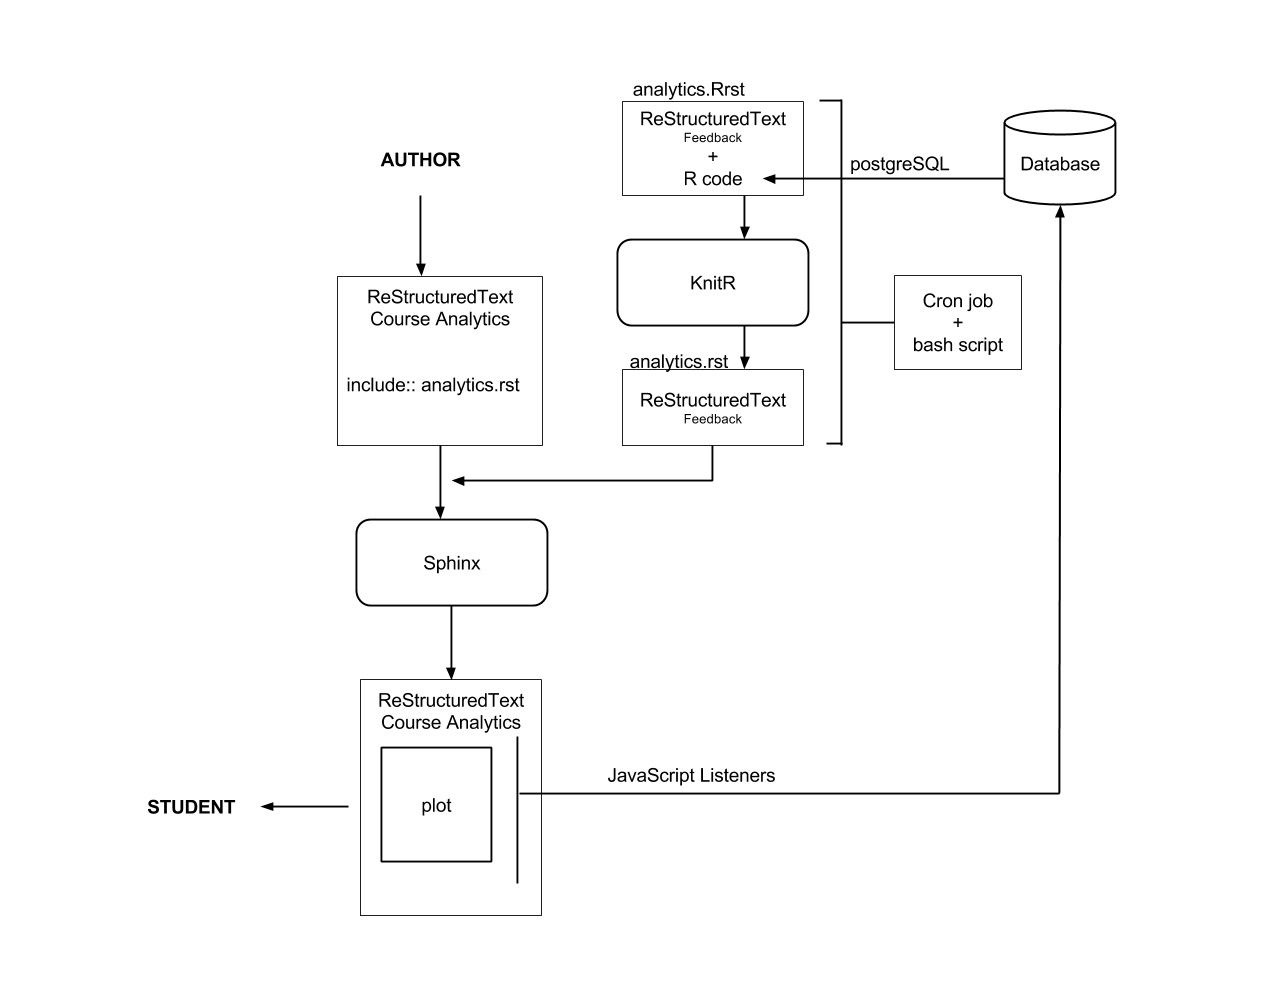
\includegraphics[width=0.6\textwidth]{loop.png}
\caption{\label{fig:loop}Diagram of the back-annotation loop}
\end{figure}

The power of the Sphinx tool lies in its ability to create web content without any assistance from the author. This is possible via the extensions which are executed when the sphinx tool identifies custom directives on the parsed reStructuredText. Asides from creating web content and JavaScript listeners, the extension also generates the unique Rrst file that will process the corresponding meta-data. This completes the automation that allows the author's contribution to simply be the directive statement in the reStructuredText file.

\section{The Importance Of Visual Analytics In Learning}

Analytics combined with effective visualization add powerful depth to online educational courses that are presently lacking in general courses. Most institutional based online courses consider visual analytics as a key component to learning and invest heavily in this area. Our education tool strives to not only provide this automatically but also such that it brings benefit to all parties, devoid of the financial limitations.

Visual analytics in learning provides a holistic system to help students gauge their progress not only through assessment tasks, but through implicit data obtained from non-assessable tasks (such as viewing specific online material). This analysis is additionally helpful for academic tutors to assess which students need more attention, and in which specific areas. Co-coordinators can observe if it is necessary to add or alter resources to meet the requirements of the class, and evaluate the correlation between engagement and performance. Researchers can further use the data to conduct specific studies pitting multiple variables against grades. A type of plot beneficial to research would be the representation of the time of day students generally view the material as shown in Figure \ref{fig:timeofday}.

\begin{figure}
\centering
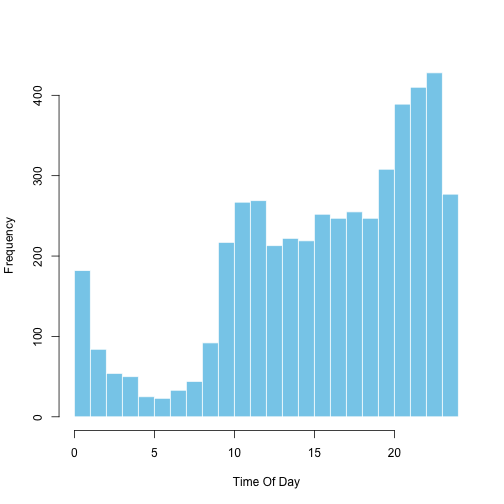
\includegraphics[width=0.45\textwidth]{timeofday.png}
\caption{\label{fig:timeofday}Distribution of study sessions throughout the day}
\end{figure}

Visuals are more engaging and give more meaningful representation of data than static feedback. 
Visuals should revolve around the students' progress and engagement, and all visuals aimed at student feedback should work as a means of positive reinforcement. Visuals that compare the performance or engagement level of a student compared to the class average have significant impact on improving performance. Too many visuals, on the other hand, cause unnecessary clutter and cloud what information is relevant to the students. Thus it is important for the tool to generate limited visuals, ranging from a fine-grained to a general level. For instance, this would include visuals depicting the effort made by the student to watch one particular video as shown in Figure \ref{fig:videoduration}, as well as those showing the number of videos watched by the student each week.

\begin{figure}
\centering
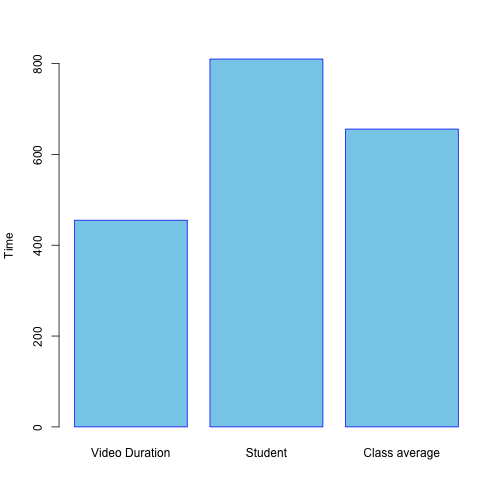
\includegraphics[width=0.45\textwidth]{videoduration.png}
\caption{\label{fig:videoduration}Time spent watching a video by a student vs. the class average}
\end{figure}

\section{Conclusion}
This education tool provides the novice author an automated online platform to make enhanced course material available to students without the need for time-consuming manual site creation and management. Expanding upon the capacity of existing online education platforms to make study material accessible online, the tool goes further to provide to students and tutors relevant performance and usage statistics designed to yield easily interpretable and meaningful visual feedback. (You'll need to write some more blah here...)

%%%%%%%%%%%%%%%%%%%%%%%%%%%%%%%%%%%%%%%%%%%%%%%%%%%%%%%%%%%%%%%%%%%%%%%%%%%%%%%%
%\section*{APPENDIX}
%Appendixes should appear before the acknowledgment.
%%%%%%%%%%%%%%%%%%%%%%%%%%%%%%%%%%%%%%%%%%%%%%%%%%%%%%%%%%%%%%%%%%%%%%%%%%%%%%%%
%References are important to the reader; therefore, each citation must be complete and correct. If at all possible, references should be commonly available publications.
%\begin{thebibliography}{99}
%\bibitem{c1} G. O. Young, ÒSynthetic structure of industrial plastics (Book style with paper title and editor),Ó 	in Plastics, 2nd ed. vol. 3, J. Peters, Ed.  New York: McGraw-Hill, 1964, pp. 15Ð64.
%\bibitem{c2} W.-K. Chen, Linear Networks and Systems (Book style).	Belmont, CA: Wadsworth, 1993, pp. 123Ð135.
%\end{thebibliography}


\end{document}
